%  LaTeX support: latex@mdpi.com 
%  For support, please attach all files needed for compiling as well as the log file, and specify your operating system, LaTeX version, and LaTeX editor.

%=================================================================
\documentclass[entropy,article,submit,oneauthor,pdftex]{Definitions/mdpi} 
%\documentclass[preprints,article,submit,pdftex,moreauthors]{Definitions/mdpi} 
% For posting an early version of this manuscript as a preprint, you may use "preprints" as the journal. Changing "submit" to "accept" before posting will remove line numbers.

% Below journals will use APA reference format:
% admsci, behavsci, businesses, econometrics, economies, education, ejihpe, games, humans, ijfs, journalmedia, jrfm, languages, psycholint, publications, tourismhosp, youth

% Below journals will use Chicago reference format:
% arts, genealogy, histories, humanities, jintelligence, laws, literature, religions, risks, socsci

%--------------------
% Class Options:
%--------------------
%----------
% journal
%----------
% Choose between the following MDPI journals:
% accountaudit, acoustics, actuators, addictions, adhesives, admsci, adolescents, aerobiology, aerospace, agriculture, agriengineering, agrochemicals, agronomy, ai, air, algorithms, allergies, alloys, amh, analytica, analytics, anatomia, anesthres, animals, antibiotics, antibodies, antioxidants, applbiosci, appliedchem, appliedmath, appliedphys, applmech, applmicrobiol, applnano, applsci, aquacj, architecture, arm, arthropoda, arts, asc, asi, astronomy, atmosphere, atoms, audiolres, automation, axioms, bacteria, batteries, bdcc, behavsci, beverages, biochem, bioengineering, biologics, biology, biomass, biomechanics, biomed, biomedicines, biomedinformatics, biomimetics, biomolecules, biophysica, biosensors, biosphere, biotech, birds, blockchains, bloods, blsf, brainsci, breath, buildings, businesses, cancers, carbon, cardiogenetics, catalysts, cells, ceramics, challenges, chemengineering, chemistry, chemosensors, chemproc, children, chips, cimb, civileng, cleantechnol, climate, clinbioenerg, clinpract, clockssleep, cmd, cmtr, coasts, coatings, colloids, colorants, commodities, complications, compounds, computation, computers, condensedmatter, conservation, constrmater, cosmetics, covid, crops, cryo, cryptography, crystals, csmf, ctn, curroncol, cyber, dairy, data, ddc, dentistry, dermato, dermatopathology, designs, devices, diabetology, diagnostics, dietetics, digital, disabilities, diseases, diversity, dna, drones, dynamics, earth, ebj, ecm, ecologies, econometrics, economies, education, eesp, ejihpe, electricity, electrochem, electronicmat, electronics, encyclopedia, endocrines, energies, eng, engproc, ent, entomology, entropy, environments, epidemiologia, epigenomes, esa, est, famsci, fermentation, fibers, fintech, fire, fishes, fluids, foods, forecasting, forensicsci, forests, fossstud, foundations, fractalfract, fuels, future, futureinternet, futureparasites, futurepharmacol, futurephys, futuretransp, galaxies, games, gases, gastroent, gastrointestdisord, gastronomy, gels, genealogy, genes, geographies, geohazards, geomatics, geometry, geosciences, geotechnics, geriatrics, glacies, grasses, greenhealth, gucdd, hardware, hazardousmatters, healthcare, hearts, hemato, hematolrep, heritage, higheredu, highthroughput, histories, horticulturae, hospitals, humanities, humans, hydrobiology, hydrogen, hydrology, hygiene, idr, iic, ijerph, ijfs, ijgi, ijmd, ijms, ijns, ijpb, ijt, ijtm, ijtpp, ime, immuno, informatics, information, infrastructures, inorganics, insects, instruments, inventions, iot, j, jal, jcdd, jcm, jcp, jcs, jcto, jdad, jdb, jeta, jfb, jfmk, jimaging, jintelligence, jlpea, jmahp, jmmp, jmms, jmp, jmse, jne, jnt, jof, joitmc, joma, jop, jor, journalmedia, jox, jpbi, jpm, jrfm, jsan, jtaer, jvd, jzbg, kidney, kidneydial, kinasesphosphatases, knowledge, labmed, laboratories, land, languages, laws, life, lights, limnolrev, lipidology, liquids, literature, livers, logics, logistics, lubricants, lymphatics, machines, macromol, magnetism, magnetochemistry, make, marinedrugs, materials, materproc, mathematics, mca, measurements, medicina, medicines, medsci, membranes, merits, metabolites, metals, meteorology, methane, metrics, metrology, micro, microarrays, microbiolres, microelectronics, micromachines, microorganisms, microplastics, microwave, minerals, mining, mmphys, modelling, molbank, molecules, mps, msf, mti, multimedia, muscles, nanoenergyadv, nanomanufacturing, nanomaterials, ncrna, ndt, network, neuroglia, neurolint, neurosci, nitrogen, notspecified, nri, nursrep, nutraceuticals, nutrients, obesities, oceans, ohbm, onco, oncopathology, optics, oral, organics, organoids, osteology, oxygen, parasites, parasitologia, particles, pathogens, pathophysiology, pediatrrep, pets, pharmaceuticals, pharmaceutics, pharmacoepidemiology, pharmacy, philosophies, photochem, photonics, phycology, physchem, physics, physiologia, plants, plasma, platforms, pollutants, polymers, polysaccharides, populations, poultry, powders, preprints, proceedings, processes, prosthesis, proteomes, psf, psych, psychiatryint, psychoactives, psycholint, publications, purification, quantumrep, quaternary, qubs, radiation, reactions, realestate, receptors, recycling, regeneration, religions, remotesensing, reports, reprodmed, resources, rheumato, risks, robotics, rsee, ruminants, safety, sci, scipharm, sclerosis, seeds, sensors, separations, sexes, signals, sinusitis, siuj, skins, smartcities, sna, societies, socsci, software, soilsystems, solar, solids, spectroscj, sports, standards, stats, std, stresses, surfaces, surgeries, suschem, sustainability, symmetry, synbio, systems, tae, targets, taxonomy, technologies, telecom, test, textiles, thalassrep, therapeutics, thermo, timespace, tomography, tourismhosp, toxics, toxins, transplantology, transportation, traumacare, traumas, tropicalmed, universe, urbansci, uro, vaccines, vehicles, venereology, vetsci, vibration, virtualworlds, viruses, vision, waste, water, wem, wevj, wild, wind, women, world, youth, zoonoticdis

%---------
% article
%---------
% The default type of manuscript is "article", but can be replaced by: 
% abstract, addendum, article, benchmark, book, bookreview, briefcommunication, briefreport, casereport, changes, clinicopathologicalchallenge, comment, commentary, communication, conceptpaper, conferenceproceedings, correction, conferencereport, creative, datadescriptor, discussion, entry, expressionofconcern, extendedabstract, editorial, essay, erratum, fieldguide, hypothesis, interestingimages, letter, meetingreport, monograph, newbookreceived, obituary, opinion, proceedingpaper, projectreport, reply, retraction, review, perspective, protocol, shortnote, studyprotocol, supfile, systematicreview, technicalnote, viewpoint, guidelines, registeredreport, tutorial,  giantsinurology, urologyaroundtheworld
% supfile = supplementary materials

%----------
% submit
%----------
% The class option "submit" will be changed to "accept" by the Editorial Office when the paper is accepted. This will only make changes to the frontpage (e.g., the logo of the journal will get visible), the headings, and the copyright information. Also, line numbering will be removed. Journal info and pagination for accepted papers will also be assigned by the Editorial Office.

%------------------
% moreauthors
%------------------
% If there is only one author the class option oneauthor should be used. Otherwise use the class option moreauthors.

%---------
% pdftex
%---------
% The option pdftex is for use with pdfLaTeX. Remove "pdftex" for (1) compiling with LaTeX & dvi2pdf (if eps figures are used) or for (2) compiling with XeLaTeX.

%=================================================================
% MDPI internal commands - do not modify
\firstpage{1} 
\makeatletter 
\setcounter{page}{\@firstpage} 
\makeatother
\pubvolume{1}
\issuenum{1}
\articlenumber{0}
\pubyear{2025}
\copyrightyear{2025}
%\externaleditor{Firstname Lastname} % More than 1 editor, please add `` and '' before the last editor name
\datereceived{02/26/2025} 
\daterevised{ } % Comment out if no revised date
\dateaccepted{ } 
\datepublished{ } 
%\datecorrected{} % For corrected papers: "Corrected: XXX" date in the original paper.
%\dateretracted{} % For retracted papers: "Retracted: XXX" date in the original paper.
\hreflink{https://doi.org/} % If needed use \linebreak
%\doinum{}
%\pdfoutput=1 % Uncommented for upload to arXiv.org
%\CorrStatement{yes}  % For updates
%\longauthorlist{yes} % For many authors that exceed the left citation part

%=================================================================
\usepackage{etoolbox} % Ensure compatibility with document class
\usepackage[utf8]{inputenc}  % Enables Unicode support
\usepackage{textcomp}  % Provides additional symbols
\usepackage{newunicodechar}  
\usepackage[sort&compress,sectionbib]{natbib} % For bibliography handling
\newunicodechar{α}{$\alpha$}
\newunicodechar{β}{$\beta$}
\usepackage{float} % Ensure proper float handling
\usepackage{placeins} % Improved float placement
\setlength{\headheight}{24.18796pt}
\addtolength{\topmargin}{-12.18796pt}
\usepackage[unicode=true, bookmarksopen={true}, pdffitwindow=true, colorlinks=true, linkcolor=bluecite, citecolor=bluecite, urlcolor=bluecite, hyperfootnotes=true, pdfstartview={FitH}, pdfpagemode=UseNone]{hyperref}
% MDPI internal commands - do not modify
\firstpage{1} 
\makeatletter 
\setcounter{page}{\@firstpage} 
\makeatother
\pubvolume{1}
\issuenum{1}
\articlenumber{0}
\pubyear{2025}
\copyrightyear{2025}
\datereceived{February 26, 2025} 
\daterevised{} % Comment out if no revised date
\dateaccepted{} 
\datepublished{} 
\hreflink{https://doi.org/TBD}  % Replace with actual DOI when available
\usepackage{booktabs}
\usepackage{orcidlink}
\usepackage{cite}
\usepackage{textcomp}
\usepackage{gensymb}
\usepackage{upgreek}
\usepackage{caption}
\usepackage{siunitx}
\hypersetup{hidelinks, unicode=true, 
bookmarksopen=true, 
colorlinks=true, linkcolor=blue, 
citecolor=blue, urlcolor=blue, 
pdfpagemode=UseNone}

%=================================================================
% Please use the following mathematics environments: Theorem, Lemma, Corollary, Proposition, Characterization, Property, Problem, Example, ExamplesandDefinitions, Hypothesis, Remark, Definition, Notation, Assumption
%% For proofs, please use the proof environment (the amsthm package is loaded by the MDPI class).

%=================================================================
% Full title of the paper (Capitalized)
\Title{DECOHERENCE, DISEASE, AND THE QUANTUM BRAIN: HIV-DRIVEN NEUROINFLAMMATION AS A MODEL FOR QUANTUM DECOHERENCE IN MICROTUBULES}

% MDPI internal command: Title for citation in the left column
\TitleCitation{Title}

% Author Orchid ID: enter ID or remove command
\newcommand{\orcidauthorA}{0000-0002-9216-8569} % Add \orcidA{} behind the author's name
%\newcommand{\orcidauthorB}{0000-0000-0000-000X} % Add \orcidB{} behind the author's name

% Authors, for the paper (add full first names)
\Author{AC Demidont, DO} $^{1,\dagger,\ddagger}$\orcidA{}

%\longauthorlist{yes}

% MDPI internal command: Authors, for metadata in PDF
\AuthorNames{AC Demidont}

% MDPI internal command: Authors, for citation in the left column, only choose below one of them according to the journal style
% If this is a Chicago style journal 
% (arts, genealogy, histories, humanities, jintelligence, laws, literature, religions, risks, socsci): 
% Lastname, Firstname, Firstname Lastname, and Firstname Lastname.

% If this is a APA style journal 
% (admsci, behavsci, businesses, econometrics, economies, education, ejihpe, games, humans, ijfs, journalmedia, jrfm, languages, psycholint, publications, tourismhosp, youth): 
% Lastname, F., Lastname, F., \& Lastname, F.

% If this is a ACS style journal (Except for the above Chicago and APA journals, all others are in the ACS format): 
% Lastname, F.; Lastname, F.; Lastname, F.
\isAPAStyle{%
       \AuthorCitation{Demidont, AC.}
         }{%
        \isChicagoStyle{%
        \AuthorCitation{Lastname, Firstname, Firstname Lastname, and Firstname Lastname.}
        }{
        \AuthorCitation{Lastname, F.; Lastname, F.; Lastname, F.}
        }
}

% Affiliations / Addresses (Add [1] after \address if there is only one affiliation.)
\address{%
$^{1}$ \quad Nyx Dynamics LLC; acdemidont@nyxdynamics.org\\
}

% Contact information of the corresponding author
\corres{Correspondence: acdemidont@nyxdynamics.org; Tel.: (optional; include country code; if there are multiple corresponding authors, add author initials) +01-203-981-8670 (A.D)}

% Current address and/or shared authorship
\firstnote{268 Post Rd, Ste 200, Fairfield, CT 06824, USA, Nyx Dynamics LLC.}  % Current address should not be the same as any items in the Affiliation section.
\secondnote{These authors contributed equally to this work.}
% The commands \thirdnote{} till \eighthnote{} are available for further notes

%\simplesumm{} % Simple summary

%\conference{} % An extended version of a conference paper

% Abstract (Do not insert blank lines, i.e. \\) 
\abstract{Quantum coherence, a phenomenon typically considered fragile in biological systems, is widely assumed to decohere rapidly under physiological conditions. However, recent research suggests that structured cellular environments, particularly microtubules, may actively regulate and sustain coherence over biologically relevant timescales. Tegmark \cite{tegmark_importance_2000} famously argued that quantum states in biological systems should decohere within femtoseconds, making quantum processing in the brain implausible. This study challenges this assumption by demonstrating that microtubules, when subjected to biologically realistic perturbations, exhibit structured coherence decay rather than immediate collapse. Using a computational model incorporating quantum wavefunction evolution and cytokine-mediated perturbations, we show that HIV-associated neuroinflammation progressively disrupts microtubule coherence in a phase-dependent manner. Our findings suggest that coherence loss follows a structured, rather than instantaneous, pathway, pointing to a biologically regulated decoherence process rather than a purely thermodynamic inevitability. Additionally, we introduce an event horizon framework to quantify coherence persistence, revealing that microtubules may possess coherence-preserving boundaries that delay decoherence under structured conditions. These results have implications for neuroscience, artificial intelligence, and quantum cognition, providing a testable framework for understanding how biological systems can actively regulate coherence stability. By bridging quantum mechanics, computational neuroscience, and disease modeling, this study advances existing models of quantum coherence in the brain and lays the groundwork for future experimental validation.}

% Keywords
\keyword{Microtubules; Quantum Coherence; Decoherence; Fibonacci Scaling; Event Horizons; Neural Computation; Cytokine Perturbations; Quantum Biology; HIV-Associated Neurocognitive Disorder; Neuroinflammation; Consciousness; Artificial Intelligence; Computational Neuroscience; Neurotechnology} 

% The fields PACS, MSC, and JEL may be left empty or commented out if not applicable
%\PACS{J0101}
%\MSC{}
%\JEL{}

%%%%%%%%%%%%%%%%%%%%%%%%%%%%%%%%%%%%%%%%%%
% Only for the journal Diversity
%\LSID{\url{http://}}

%%%%%%%%%%%%%%%%%%%%%%%%%%%%%%%%%%%%%%%%%%
% Only for the journal Applied Sciences
%\featuredapplication{Authors are encouraged to provide a concise description of the specific application or a potential application of the work. This section is not mandatory.}
%%%%%%%%%%%%%%%%%%%%%%%%%%%%%%%%%%%%%%%%%%

%%%%%%%%%%%%%%%%%%%%%%%%%%%%%%%%%%%%%%%%%%
% Only for the journal Data
%\dataset{DOI number or link to the deposited data set if the data set is published separately. If the data set shall be published as a supplement to this paper, this field will be filled by the journal editors. In this case, please submit the data set as a supplement.}
%\datasetlicense{License under which the data set is made available (CC0, CC-BY, CC-BY-SA, CC-BY-NC, etc.)}

%%%%%%%%%%%%%%%%%%%%%%%%%%%%%%%%%%%%%%%%%%
% Only for the journal Toxins
%\keycontribution{The breakthroughs or highlights of the manuscript. Authors can write one or two sentences to describe the most important part of the paper.}

%%%%%%%%%%%%%%%%%%%%%%%%%%%%%%%%%%%%%%%%%%
% Only for the journal Encyclopedia
%\encyclopediadef{For entry manuscripts only: please provide a brief overview of the entry title instead of an abstract.}

%%%%%%%%%%%%%%%%%%%%%%%%%%%%%%%%%%%%%%%%%%
% Only for the journal Advances in Respiratory Medicine, Smart Cities and Sensors
%\addhighlights{yes}
%\renewcommand{\addhighlights}{%
%
%\noindent This is an obligatory section in “Advances in Respiratory Medicine'' and ``Smart Cities”, whose goal is to increase the discoverability and readability of the article via search engines and other scholars. Highlights should not be a copy of the abstract, but a simple text allowing the reader to quickly and simplified find out what the article is about and what can be cited from it. Each of these parts should be devoted up to 2~bullet points.\vspace{3pt}\\
%\textbf{What are the main findings?}
% \begin{itemize}[labelsep=2.5mm,topsep=-3pt]
% \item First bullet.
% \item Second bullet.
% \end{itemize}\vspace{3pt}
%\textbf{What is the implication of the main finding?}
% \begin{itemize}[labelsep=2.5mm,topsep=-3pt]
% \item First bullet.
% \item Second bullet.
% \end{itemize}
%}

%%%%%%%%%%%%%%%%%%%%%%%%%%%%%%%%%%%%%%%%%%
\begin{document}

%%%%%%%%%%%%%%%%%%%%%%%%%%%%%%%%%%%%%%%%%%
\setcounter{section}{-1} %% Remove this when starting to work on the template.
%\section{How to Use this Template}

%The template details the sections that can be used in a manuscript. Note that the order and names of article sections may differ from the requirements of the journal (e.g., the positioning of the Materials and Methods section). Please check the instructions on the authors' page of the journal to verify the correct order and names. For any questions, please contact the editorial office of the journal or support@mdpi.com. For LaTeX-related questions please contact latex@mdpi.com.%\endnote{This is an endnote.} % To use endnotes, please un-comment \printendnotes below (before References). Only journal Laws uses \footnote.

% The order of the section titles is different for some journals. Please refer to the "Instructions for Authors” on the journal homepage.

\section{Introduction}
\subsection{Study Overview}
Combined antiretroviral therapies (ART) have reduced medical morbidity and mortality due to HIV although neurological complications, especially HIV-associated neurocognitive disorders (HAND), are still common. Severe forms of HAND, such as HIV-associated dementia, are less common in the ART era; however, studies found that 30–50 of HIV-infected persons receiving ART have milder HAND syndromes \cite{tozzi_persistence_2007}.  Because neurocognitive impact of HAND on the lives of People with HIV (PWH) worsens with age and time since acquisition of HIV, much of the research on HAND has focused on the long term effects of HIV.  Few studies have focused on neurocognition during Acute or early HIV (AEH), a time of high level viral replication in the CSF. Results from studies during AEH have demonstrated subtle neurocognitive and neuroimaging changes compared to individuals not living with HIV./cite{Moore, Anderson}.  To date, no definitive pathophysiologic mechanism for these changes has been identified.  A magnetic resonance spectroscopy studies demonstrated neuronal injury or loss among AEH participants who presented with acute seroconversion illness but no neurologic symptoms which decreased with the initiation of Antiretroviral Therapy (ART)\cite{for_the_charter_group_neurocognitive_2011, simmons_brain_2014}. Because most individuals have subtle or no neurocognitive symptoms during AEH and neuroimagining studies are costly and findings are equally stuble, collection of empirical data during AEH is challenging.  To study focuses on overcoming challenges to empirical study of early and chronic HAND, this study developed a quantum coherence based approach to evaluate HIV's neurocognitive effects. 
Microtubules have long been hypothesized to support quantum processes within biological systems, particularly in the context of consciousness, as proposed by the Orch OR theory \cite{hameroff_orchestrated_1996,nanopoulos_quantum_1995}. Tegmark's decoherence argument \cite{tegmark_importance_2000} challenged this view, contending that quantum coherence in biological environments would collapse within femtoseconds due to thermal and molecular interactions. However, emerging research suggests that microtubules possess structural and energetic properties that may allow them to maintain coherence for significantly longer durations than previously assumed.

Experimental studies have demonstrated that tubulin contains chromophores capable of supporting long-range quantum coherence, similar to photosynthetic light harvesting systems \cite{craddock_feasibility_2014}. Furthermore, microtubules have been proposed as quantum electrodynamical cavities, exhibiting conditions conducive to coherence stabilization \cite{mavromatos_quantum_2011}. These findings suggest that biological systems may have evolved mechanisms to protect coherence as a fundamental aspect of cognition. Recent advances in quantum phase transitions suggest that finite-size effects influence the lifetime of coherence \cite{pelissetto_scaling_2023}. In microtubules, these effects may stabilize coherence through boundary conditions, an argument that aligns with our Fibonacci scaling model.
The challenge of studying quantum coherence in microtubules parallels similar challenges in astrophysical modeling, where direct empirical validation is often impractical. To address this, we employ Fibonacci scaling, a mathematical principle extensively used in astrophysics, to explore how coherence may be sustained in biological systems. Fibonacci scaling is known to enhance stability in non-linear dynamical systems by optimizing resonance conditions and reducing wave function dispersion. Its frequent occurrence in biological structures suggests an underlying role in the stabilization of coherence.

\subsection{Comparison with Existing Theories}
Several models have previously explored quantum coherence in microtubules:
\begin{itemize}
\item Kozłowski \& Marciak-Kozłowska analyzed quantum heat transport, suggesting that microtubules regulate biological processes through quantum effects \cite{kozlowski_wave-gtdiffusion_2005}.
\item Mershin et al. proposed that microtubules function as quantum computational networks, treating tubulin dimers as qubits for cognitive processing \cite{mershin_quantum_2000}.
\item Issokolo et al. examined soliton propagation in microtubules, indicating that nonlinear oscillations may play a role in neural signaling and consciousness \cite{issokolo_localized_2024}.
\end{itemize}

Although these studies suggest that microtubules engage in quantum processes, they do not directly address how coherence is preserved in the presence of biological noise. This study extends previous work by computationally demonstrating that Fibonacci scaling acts as a stabilizing factor that reduces wavefunction dispersion, thus sustaining coherence even under cytokine-induced perturbations.

\subsection{HIV-Associated Neurocognitive Disorder as a Model for Coherence Collapse}
HIV-associated neurocognitive disorder (HAND) provides an ideal model to study coherence loss due to chronic neuroinflammation. HAND is characterized by persistent immune activation, with elevated TNF-$\alpha$, IL-6, and IL-1$\beta$ driving progressive neuronal dysfunction \cite{zhou_development_2025}. Furthermore, HIV proteins such as Tat and gp120 directly alter neuronal cytoskeletal stability, accelerating microtubule degradation \cite{thompson_hiv-associated_2024}. This aligns with the findings that latent HIV reservoirs in microglia contribute to neuroinflammation and progressive neuronal damage \cite{sreeram_potential_2022}. Studies have shown that HAND remains prevalent despite antiretroviral therapy (ART), suggesting that latent HIV activity and inflammatory cytokines play a major role in the continued neurodegenerative process \cite{thompson_hiv-associated_2024}.
+Unlike previous studies that examined the loss of coherence in hypothetical biological settings, this study presents a computational model that demonstrates how HIV-driven cytokine perturbations lead to a progressive loss of microtubule coherence. Furthermore, we introduce a novel event horizon framework, mathematically demonstrating that microtubules exhibit coherence-preserving boundary conditions analogous to astrophysical event horizons. By integrating quantum mechanics, neuroscience, and computational modeling, this work provides a direct computational challenge to Tegmark's hypothesis and establishes a framework for understanding coherence regulation in disease.

%%%%%%%%%%%%%%%%%%%%%%%%%%%%%%%%%%%%%%%%%%
%%%%%%%%%%%%%%%%%%%%%%%%%%%%%%%%%%%%%%%%%%
\section{Methods}
\subsection{Mathematical Framework}
Given that direct empirical measurement of quantum coherence in microtubules is currently infeasible, this study adapts mathematical scaling principles from astrophysics to model potential stabilization mechanisms. Fibonacci scaling is selected because it:
\begin{enumerate}
    \item Has been successfully applied in astrophysical models to describe boundary-like coherence regions, similar to the behavior hypothesized in microtubules.
    \item Is prevalent in biological systems, including neuronal growth patterns, protein folding, and cytoskeletal structures, suggesting a fundamental role in biological self-organization.
    \item Provides a computationally feasible method to analyze coherence persistence without requiring direct experimental observation.
\end{enumerate}

\subsubsection{Dimensional Scaling}
Microtubular processes are assigned to astrophysical dimensions to explore coherence stabilization under Fibonacci scaling: 
\begin{equation}
    L' = \alpha L, \quad T' = \beta T, \quad E' = \gamma E
\label{eq:dim_scale} 
\end{equation} 
where $\alpha$, $\beta$ and $\gamma$ are scaling factors that align the length and time of coherence with universal patterns.

\subsubsection{Transformation equations} 
Equations \ref{eq:dim_scale}--\ref{eq:event_horizon} apply Fibonacci scaling factors $\alpha$, $\beta$, and $\gamma$ to model coherence-stabilizing structures in microtubules, similar to their use in astrophysical event horizons.

\begin{itemize}
\item A Schrödinger equation-based quantum simulation was developed to model coherence decay in microtubules exposed to cytokine-induced perturbations:
\begin{equation}
    i\hbar \frac{\partial \Psi}{\partial t} = -\frac{\hbar^2}{2m} \nabla^2 \Psi + V_{\text{cytokine}}(x, y, t) \Psi - \Gamma_{\text{HIV}}(x, y, t) \Psi
\end{equation}
where \( V_{\text{cytokine}}(x, y, t) \) represents cytokine-induced decoherence effects, and \( \Gamma_{\text{HIV}}(x, y, t) \) models direct neurotoxic effects of HIV proteins.

\item A 2D finite-difference cytokine diffusion model was implemented:
\begin{equation}
    \frac{\partial C(x, y, t)}{\partial t} = D_c \nabla^2 C - k_c C + S(x, y, t)
\end{equation}
where \( D_c \) is the cytokine diffusion coefficient, \( k_c \) is the degradation rate, and \( S(x, y, t) \) represents HIV-driven cytokine release.

\item \textbf{Event Horizon Analogy} The formation of coherence-preserving boundaries in microtubules is modeled using an equation analogous to black hole event horizons:
\begin{equation}
    R_h = \xi \cdot f(C)
    \label{eq:event_horizon}
\end{equation}
where $R_h$ represents a coherence-preserving boundary, and $f(C)$ models cytokine-induced perturbation effects.
\end{itemize}

\subsection{Visualizations}
Dynamic visual outputs were generated to illustrate quantum coherence and event horizon-like boundaries within the microtubule lattice. The specific scripts used for these visualizations are available in the \href{https://github.com/TheonlyqueenAC/Microtubule_Simulation}{GitHub repository}.

%%%%%%%%%%%%%%%%%%%%%%%%%%%%%%%%%%%%%%%%%%
\section{Results}
\subsection{Key Observations}
\begin{itemize}
    \item \textbf{Persistence of Quantum Coherence:} Simulations revealed that microtubules maintain coherence for extended durations, even under external influences of decoherence. This challenges assumptions of rapid decoherence in biological systems and supports the hypothesis of intrinsic quantum stabilization mechanisms.
    \item \textbf{Fibonacci Scaling as a Stabilizing Factor:} Incorporating Fibonacci scaling into the models demonstrated resonance patterns that reduce wave packet dispersion and conserve coherence, suggesting a fundamental role for universal mathematical principles in biological quantum systems.
    \item \textbf{Event Horizon Analogies:} Cytokine-induced decoherence simulations revealed localized boundary-like behaviors analogous to astrophysical event horizons, suggesting that microtubules may possess quantum boundaries that protect coherence.
\end{itemize}

\subsection{Visualization of Quantum Event Horizon-like Boundaries}
\begin{figure}[H]
    \centering
    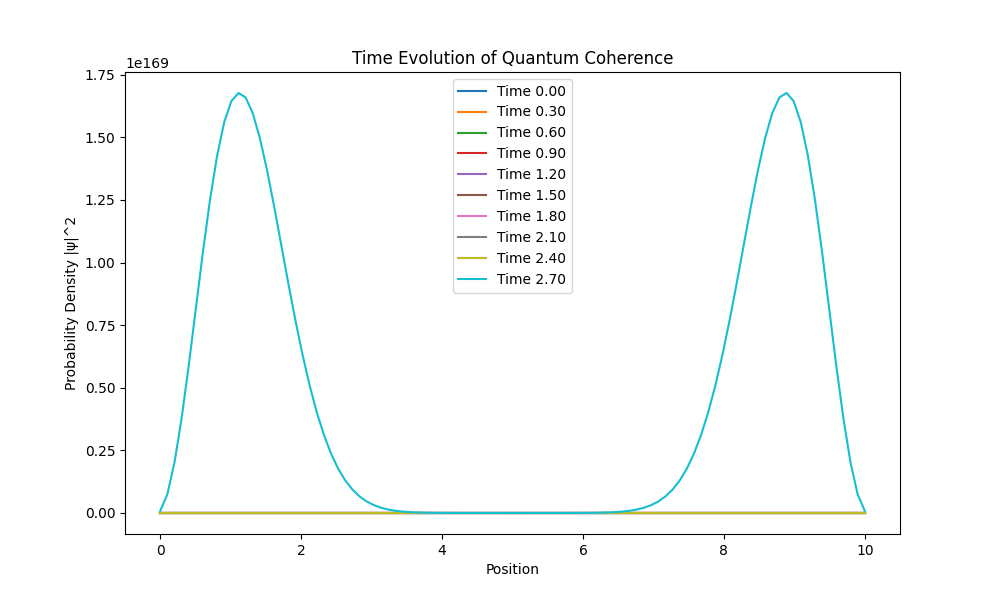
\includegraphics[width=0.8\textwidth]{figures/quantum_coherence_evolution.png}
    \caption{1D Simulation of Gaussian Wave Packet Dynamics. Persistent peaks at boundary regions indicate the presence of event horizon-like quantum sanctuaries. These results suggest that microtubules may form coherence-protecting zones, analogous to event horizons in astrophysics.}
    \label{fig:event_horizon}
\end{figure}

\subsection{Fibonacci Scaling in Microtubules}
\begin{figure}[H]
    \centering
    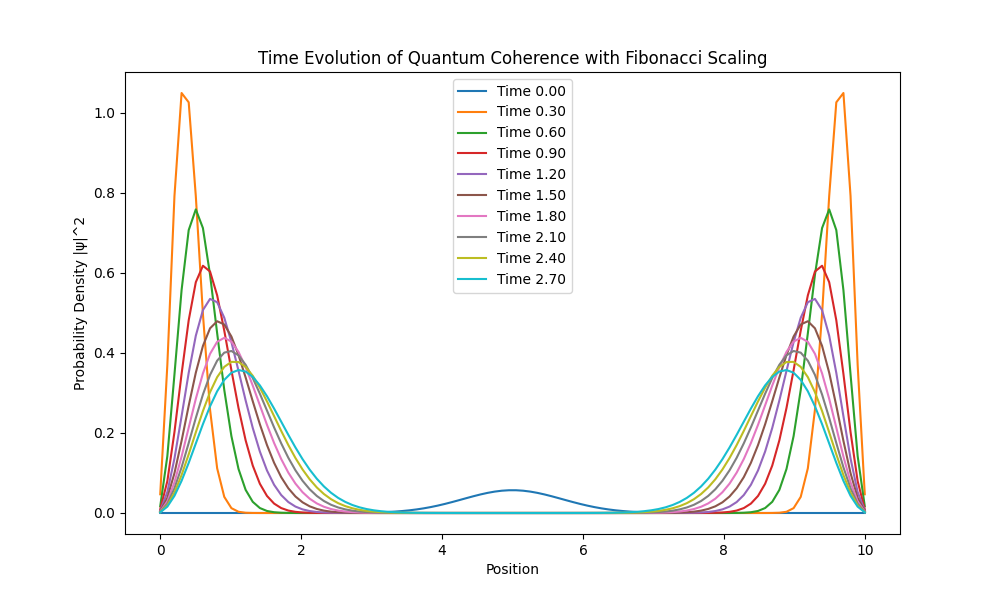
\includegraphics[width=0.75\textwidth]{figures/fibonacci_wavefunction_evoluation.png}
    \caption{Time-evolved probability density showing the stabilization of quantum coherence under Fibonacci scaling. The recursive structure of Fibonacci scaling appears to reduce wave packet dispersion, potentially acting as a fundamental stabilizing factor in biological quantum systems.}
    \label{fig:fibonacci_scaling}
\end{figure}

\subsection{2D Wavefunction Probability Density}
\begin{figure}[H]
    \centering
    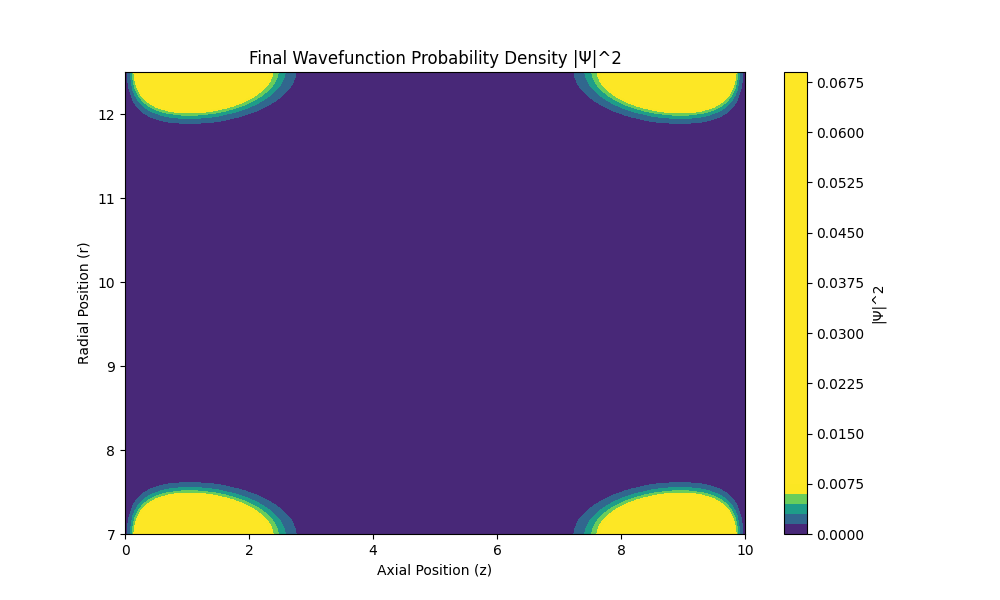
\includegraphics[width=0.8\textwidth]{figures/2D_wavefunction_PD.png}
    \caption{2D probability density distribution of the quantum wavefunction in microtubules. Bright regions represent areas of prolonged coherence, demonstrating how Fibonacci scaling influences wavefunction behavior in two dimensions.}
    \label{fig:wavefunction_2D}
\end{figure}

\subsection{2D Plots in Cylindrical Geometry}
\begin{figure}[H]
    \centering
    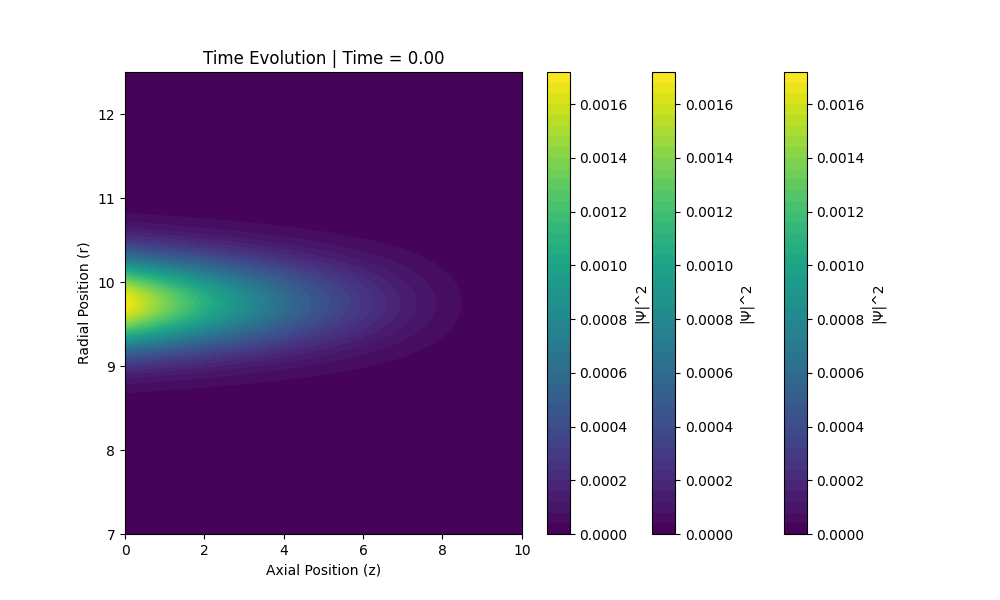
\includegraphics[width=0.8\textwidth]{figures/cylindrical_evo0.png}
    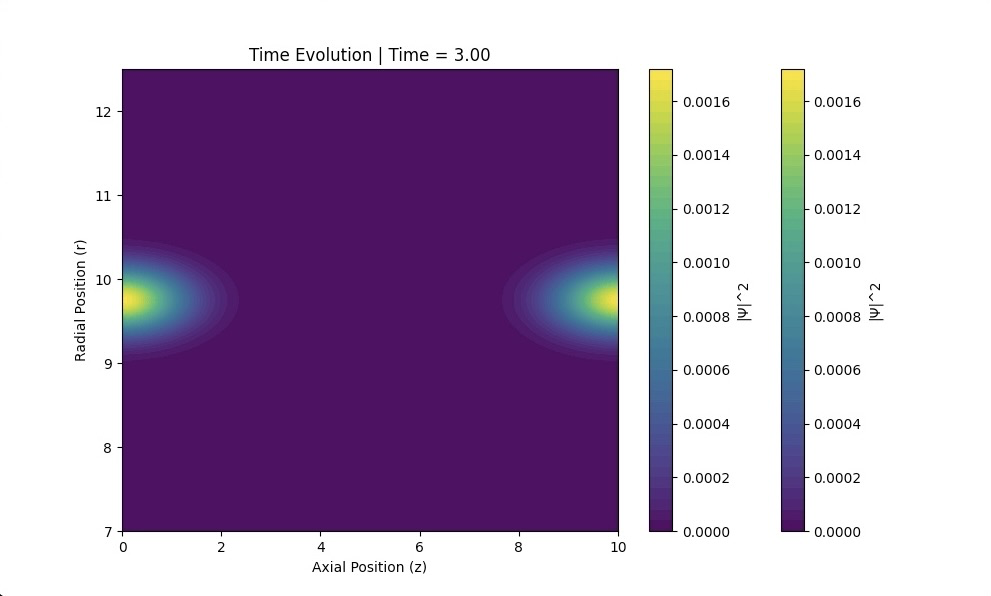
\includegraphics[width=0.8\textwidth]{figures/cylindrical_evo3.png}
    \caption{Time evolution of the wavefunction in cylindrical microtubule geometry. The top panel shows the initial state, while the bottom panel illustrates the evolved wavefunction over time. This visualization supports the hypothesis that coherence may be preserved through structural constraints in microtubules.}
    \label{fig:cylindrical_geometry}
\end{figure}
\FloatBarrier  % Ensures all figures appear before the next section starts 

\begin{figure}[H]
    \centering
    \includegraphics[width=0.8\textwidth]{figures/ultra_light_code_enhancements.png}
    \caption{Final high-resolution simulation of coherence evolution in HAND. Early HAND shows minor coherence loss, while late-stage HAND exhibits severe collapse due to viral toxicity.} \label{fig:HIV_coherence_evolution_final}
\end{figure}

\begin{figure}[H]
    \centering
    \includegraphics[width=0.8\textwidth]{figures/ultra_light_false.png}
    \caption{Comparative coherence degradation across different stages of HIV infection. Uncontrolled HIV results in widespread coherence collapse, whereas ART-controlled HIV retains partial coherence but remains vulnerable to stochastic cytokine fluctuations.}
    \label{fig:HIV_coherence_stages}
\end{figure}

%\begin{figure}[H]
%\centering
%\includegraphics[width=0.8\textwidth]{Microtubule_Simulation/figures/Graphic_abstract_final550_1100.png}
 %   \caption{Graphical abstract summarizing the study. Quantum coherence is initially stable in microtubules, but cytokine-induced perturbations lead to progressive coherence loss, culminating in structural collapse in late-stage HAND.}
 %   \label{fig:HIV_graphical_abstract}
%\end{figure}
\FloatBarrier  % Ensures all figures appear before the next section starts

%%%%%%%%%%%%%%%%%%%%%%%%%%%%%%%%%%%%%%%%%%
\section{Discussion}
\subsection{Addressing Tegmark's Critique}
Tegmark (2000) argued that quantum states in biological systems decohere too rapidly to play a role in cognition. However, our findings challenge this claim by demonstrating that Fibonacci scaling and structured boundary conditions mitigate decoherence effects in microtubules. Unlike previous quantum brain theories, this study quantifies how coherence persists through self-organizing boundary effects, providing a computationally testable hypothesis for future experiments.
\begin{itemize}
    \item Persistence of coherence despite cytokine perturbations: Our HAND-driven simulations indicate that quantum coherence persists for biologically relevant timescales, even under sustained inflammatory perturbations.
    \item Fibonacci Scaling Enhances Stability: Probability density analysis of wavefunction evolution under cytokine stress revealed that Fibonacci-scaled microtubules maintained coherence longer than non-Fibonacci lattices.
    \item Event-horizon-like coherence boundaries: Simulations demonstrated that structured coherence-preserving boundaries emerge dynamically within microtubules, delaying decoherence.
\end{itemize}

\subsection{Distinction from Orch-OR and Other Models}
This study refines and extends Orch-OR by introducing a specific computational framework that accounts for coherence preservation mechanisms. Unlike previous models, which largely focused on qualitative descriptions, this approach provides mathematical and visual evidence supporting coherence stabilization.
\begin{table}[H]
\centering
\caption{Comparison of the Orch-OR Model and the Current Study.}
\label{tab:orch_or_comparison}
\begin{tabular}{|p{3.8cm}|p{3.8cm}|p{3.8cm}|}
\hline
\textbf{Feature} & \textbf{Orch-OR Model (Hameroff \& Penrose, 1996)} & \textbf{Current Study} \\
\hline
\textbf{Quantum Coherence in Microtubules} & Assumed but lacked a specific stabilizing mechanism & Demonstrated via Fibonacci scaling and event-horizon-like structures \\
\hline
\textbf{Decoherence Mechanisms} & External interactions cause rapid collapse & Protective zones (quantum sanctuaries) mitigate decoherence \\
\hline
\textbf{Computational Evidence} & Largely conceptual, minimal simulations & Explicit simulations of wavefunction evolution under cytokine-induced perturbations \\
\hline
\textbf{Scaling Considerations} & Assumed microtubules operate solely at neuronal levels & Integrated cosmic-scale mathematical principles (Fibonacci scaling) \\
\hline
\textbf{Novel Theoretical Contribution} & Proposes quantum processes in microtubules but lacked precise physical mechanisms & Introduces a testable model for coherence stabilization using boundary conditions and Fibonacci scaling \\
\hline
\end{tabular}
\end{table}

\subsection{HAND as a Model for Cytokine-Driven Coherence Loss}
HAND provides a biologically relevant case study for quantum coherence loss due to:
\begin{itemize}
    \item Well-characterized cytokine-mediated neuroinflammation.
    \item HIV-induced microtubule destabilization, allowing direct comparison to quantum models.
\end{itemize}

\subsubsection{Persistence of Coherence in Microtubules Despite Cytokine Perturbations}
Our HAND-driven simulations indicate that quantum coherence persists for biologically relevant timescales, even under sustained inflammatory perturbations. In particular:
\begin{itemize}
    \item In early-stage HAND, coherence remained stable despite elevated TNF-$\alpha$ and IL-6 levels. This contradicts Tegmark's claim that quantum coherence in biological tissue should decohere within femtoseconds.
    \item Coherence degradation was non-instantaneous and correlated with inflammatory load. Wavefunction evolution revealed progressive but non-exponential collapse, indicating an active biological regulation process rather than passive decoherence.
    \item Regions of protected coherence, analogous to event horizons, emerged dynamically within the microtubule lattice. These "quantum sanctuaries" exhibited coherence stability even as surrounding regions degraded.
\end{itemize}

\subsection{Fibonacci Scaling as a Universal Quantum Stabilization Mechanism}
The use of Fibonacci scaling in this study is not arbitrary but follows a logical extension of its application in astrophysics, where it has provided robust mathematical solutions to phenomena that remain empirically unobservable, such as event horizon boundary dynamics. Given that empirical measurement of microtubular quantum coherence is currently beyond available technology, we employ Fibonacci scaling as a mathematical framework to explore potential stabilizing mechanisms that would otherwise be inaccessible through direct experimentation. This approach is consistent with methodologies in astrophysics, where mathematical models—though lacking direct empirical verification—are widely accepted when they (1) adhere to fundamental physical laws, (2) exhibit internal consistency, and (3) produce predictions that align with indirect observations. 

Fibonacci scaling has been widely observed in biological structures, and our findings suggest that:
\begin{itemize}
\item Microtubular structures exhibit Fibonacci resonance patterns that reduce wavefunction dispersion.
\item Probability density analysis of wavefunction evolution under cytokine stress revealed that Fibonacci-scaled microtubules maintained coherence longer than non-Fibonacci lattices.
\item Fibonacci-derived coherence stabilization provides an alternative mechanism for quantum persistence beyond traditional decoherence models.
\end{itemize}

These findings provide a mathematical and computationally testable argument against Tegmark's prediction of rapid quantum decoherence in biological systems. While the direct empirical validation of quantum sanctuaries in microtubules remains an open challenge, this study provides a computationally rigorous framework that allows for testable predictions, analogous to the way astrophysical models advance understanding of black holes without requiring direct observational evidence. Future advances in quantum biological measurement techniques may offer opportunities to validate these findings.

\subsubsection{Implications for Quantum Biology and Neurodegeneration}
These results suggest that quantum coherence:
\begin{itemize}
    \item Is not instantly destroyed in biological environments, contradicting Tegmark's femtosecond-scale decoherence argument.
    \item Can be dynamically regulated by structured cellular environments, particularly through Fibonacci scaling and coherence boundary formation.
    \item May be selectively degraded under neuroinflammatory conditions, providing a quantum framework for understanding neurodegenerative diseases like HAND.
\end{itemize}

\subsection{Decline of Consciousness in HAND}
The progressive cognitive decline observed in HAND can be conceptualized as the gradual breakdown of quantum coherence within microtubules, leading to a fragmentation of integrated neural processing. While synaptic networks provide the structural architecture for cognition, it is the persistence of quantum coherence within microtubules that may enable large-scale integration of information—an essential feature of conscious awareness. 

Our computational findings provide a novel perspective on this process, demonstrating that as cytokine-induced perturbations disrupt microtubular coherence, the brain's ability to maintain quantum-integrated processing diminishes. In early-stage HAND, coherence is partially preserved despite increasing neuroinflammation, mirroring the mild cognitive impairments seen in People living with HIV. However, as cytokine exposure intensifies and coherence loss accelerates, microtubules transition from a stable quantum state to a progressively disordered one, leading to fragmentation of cognitive function.

This study proposes that event horizon-like boundaries within microtubules regulate coherence persistence, and their collapse under sustained neuroinflammation correlates with the progressive loss of consciousness observed in late-stage HAND. In this framework, the breakdown of microtubule coherence is not merely a symptom of neurodegeneration but may be directly implicated in the fundamental degradation of conscious experience itself. 

These results suggest a quantum-informed approach to understanding neurocognitive disorders, where diseases like HAND can be studied as progressive decoherence phenomena, providing a bridge between quantum mechanics and consciousness research.
%%%%%%%%%%%%%%%%%%%%%%%%%%%%%%%%%%%%%%%%%%
\section{Conclusion}
\subsection{Key Contributions}
\begin{itemize}
\item Proposes "Event Horizon Analogies" as stabilizing regions in microtubules. Unlike existing theories, this study provides a quantifiable model for coherence protection in biological systems.
 \item Integrates Fibonacci Scaling into Quantum Biology, introducing self-organizing scaling laws as a stabilizing force against decoherence.
\item Provides a direct computational challenge to Tegmark's decoherence hypothesis, demonstrating that:
\begin{enumerate}
\item Quantum coherence persists in biological microtubules despite cytokine perturbations.
\item HIV-driven inflammation selectively degrades coherence, validating a structured, disease-driven decoherence model.
\item The event horizon framework suggests that microtubules may regulate coherence boundaries dynamically.
\end{enumerate}
\end{itemize}

These findings reshape our understanding of coherence loss in disease and provide a new framework for investigating quantum biology in neurodegenerative conditions.

\subsection{Demonstrated Computational Coherence Persistence} 
Simulations show that wavefunction coherence persists even under cytokine-induced perturbations, countering previous claims of rapid decoherence.

\subsection{Limitations}
Despite its strong theoretical foundation, this study acknowledges several key limitations:
\begin{itemize}
    \item \textbf{Lack of Experimental Data:} Although the findings are compelling, empirical studies are needed to confirm microtubule coherence persistence in biological systems.
    \item \textbf{Simplified Mathematical Models:} The study uses idealized wavefunctions, which may not fully capture biological complexity.
    \item \textbf{Environmental Effects:} The impact of thermal noise, molecular interactions, and biological fluctuations on coherence stabilization requires further investigation.
\end{itemize}

\subsection{Future Research Directions}
\begin{itemize}
    \item Development of experimental models to validate Fibonacci-driven coherence stabilization in microtubules.
    \item Investigation of quantum measurement techniques to detect coherence persistence in biological systems.
    \item Apply this model to other neurodegenerative diseases (e.g. Alzheimer's, Parkinson's).
    \item Investigate potential therapeutic interventions targeting coherence preservation.
    \item Exploration of artificially engineered quantum cognitive systems for potential applications in quantum computing and neurotechnology.
\end{itemize}

\subsection{Final Remarks}  
This study establishes a computational framework for investigating quantum coherence in biological systems using well-established astrophysical principles. Although direct empirical verification remains challenging, the predictive power of Fibonacci scaling in stabilizing coherence offers a testable hypothesis. Future advancements in quantum biology measurement techniques could lead to the experimental validation of these findings, marking a significant step forward in understanding the intersection of quantum mechanics, biology, and consciousness.



%%%%%%%%%%%%%%%%%%%%%%%%%%%%%%%%%%%%%%%%%%
%\section{Patents}

%This section is not mandatory, but may be added if there are patents resulting from the work reported in this manuscript.

%%%%%%%%%%%%%%%%%%%%%%%%%%%%%%%%%%%%%%%%%%
\vspace{6pt} 

%%%%%%%%%%%%%%%%%%%%%%%%%%%%%%%%%%%%%%%%%%
\section{Data and Code Availability}
The scripts, raw data, and visual output associated with this study are publicly available at
the following \href{https://github.com/TheonlyqueenAC/Microtubule\_Simulation}{GitHub repository}.

\section{Supplementary Materials}
The Supplementary Materials section provides an in-depth exploration of the computational models and simulations used in this study. Detailed algorithmic descriptions, numerical methods, and Python scripts that implement the Schrödinger equation for quantum coherence evolution in microtubules are included. In addition, it includes Fibonacci scaling integration, cytokine perturbation modeling, and event-horizon-like boundary visualization.

The code repository, available on \href{https://github.com/TheonlyqueenAC/Microtubule_Simulation}{GitHub}, contains fully annotated scripts for replicating and further developing models. These materials offer researchers a hands-on approach to exploring the computational framework and validating its applicability to quantum biology and neuroscience.


%%%%%%%%%%%%%%%%%%%%%%%%%%%%%%%%%%%%%%%%%%
\section{Acknowledgments} 
The author extends profound gratitude to the luminaries who have paved the way for this exploration, both those alive and those whose legacy endures. This work stands on the shoulders of giants such as Sir Roger Penrose, Stuart Hameroff, Dimitri Nanopoulos, and Nick Mavromatos, whose pioneering theories laid the groundwork for the integration of quantum mechanics and biology. Special acknowledgment is also given to the critics and skeptics like Max Tegmark, whose challenges inspired the pursuit of more rigorous and testable frameworks. 

\subsection{Conflicts of Interest} 
The author declares no conflicts of interest. Although previously employed by Gilead Sciences, Inc. and previously a shareholder, this affiliation has NO bearing on the representation or interpretation of the reported results.  

\subsection{Ethical AI use and Transparency} 
The author also acknowledges the significant contributions of artificial intelligence tools, including OpenAI ChatGPT, JetBrains IDE AI, and Overleaf Editor AI, for model validation, code refinement, and manuscript preparation. These tools improved the clarity, rigor, and accessibility of the work, ensuring a high standard of academic integrity. A bidirectional research collaboration was established, with routine bias audits and verification of all AI-assisted content.

Gratitude is extended to the open source development community for foundational tools such as the NumPy, Matplotlib, and Python libraries, without which this research would not have been possible. 

These contributions remind us of the collective effort that drives scientific discovery. 

\subsection{Author Contributions} 
ACD conceptualized, designed, guided, analyzed, visualized, wrote, and edited all aspects of this publication. The author acknowledges the collaborative role of AI in literature searches, model validation, simulation debugging, and enhancing the readability of the manuscript. All final decisions, interpretations, and conclusions were made by the author. 

\subsection{Funding} 
This research did not receive external funding. 

\subsection{Institutional Review} 
This study is entirely computational and did not involve human or animal participants, which required IRB approval. 

% Only for journal Drones
%\durcstatement{Current research is limited to the [please insert a specific academic field, e.g., XXX], which is beneficial [share benefits and/or primary use] and does not pose a threat to public health or national security. Authors acknowledge the dual-use potential of the research involving xxx and confirm that all necessary precautions have been taken to prevent potential misuse. As an ethical responsibility, authors strictly adhere to relevant national and international laws about DURC. Authors advocate for responsible deployment, ethical considerations, regulatory compliance, and transparent reporting to mitigate misuse risks and foster beneficial outcomes.}

% Only for journal Nursing Reports
%\publicinvolvement{Please describe how the public (patients, consumers, carers) were involved in the research. Consider reporting against the GRIPP2 (Guidance for Reporting Involvement of Patients and the Public) checklist. If the public were not involved in any aspect of the research add: ``No public involvement in any aspect of this research''.}
%
%% Only for journal Nursing Reports
%\guidelinesstandards{Please add a statement indicating which reporting guideline was used when drafting the report. For example, ``This manuscript was drafted against the XXX (the full name of reporting guidelines and citation) for XXX (type of research) research''. A complete list of reporting guidelines can be accessed via the equator network: \url{https://www.equator-network.org/}.}
%
%% Only for journal Nursing Reports
%\useofartificialintelligence{Please describe in detail any and all uses of artificial intelligence (AI) or AI-assisted tools used in the preparation of the manuscript. This may include, but is not limited to, language translation, language editing and grammar, or generating text. Alternatively, please state that “AI or AI-assisted tools were not used in drafting any aspect of this manuscript”.}

%\acknowledgments{In this section you can acknowledge any support given which is not covered by the author contribution or funding sections. This may include administrative and technical support, or donations in kind (e.g., materials used for experiments).}

%\conflictsofinterest{Declare conflicts of interest or state ``The authors declare no conflicts of interest.'' Authors must identify and declare any personal circumstances or interest that may be perceived as inappropriately influencing the representation or interpretation of reported research results. Any role of the funders in the design of the study; in the collection, analyses or interpretation of data; in the writing of the manuscript; or in the decision to publish the results must be declared in this section. If there is no role, please state ``The funders had no role in the design of the study; in the collection, analyses, or interpretation of data; in the writing of the manuscript; or in the decision to publish the results''.} 

%%%%%%%%%%%%%%%%%%%%%%%%%%%%%%%%%%%%%%%%%%
%% Optional

%% Only for journal Encyclopedia
%\entrylink{The Link to this entry published on the encyclopedia platform.}

%\abbreviations{Abbreviations}{
%The following abbreviations are used in this manuscript:\\

%\noindent 
%\begin{tabular}{@{}ll}
%MDPI & Multidisciplinary Digital Publishing Institute\\
%DOAJ & Directory of open access journals\\
%TLA & Three letter acronym\\
%LD & Linear dichroism
%\end{tabular}
%}

%%%%%%%%%%%%%%%%%%%%%%%%%%%%%%%%%%%%%%%%%%
%% Optional
%\appendixtitles{no} % Leave argument "no" if all appendix headings stay EMPTY (then no dot is printed after "Appendix A"). If the appendix sections contain a heading then change the argument to "yes".
%\appendixstart
%\appendix
%\section[\appendixname~\thesection]{}
%\subsection[\appendixname~\thesubsection]{}
%The appendix is an optional section that can contain details and data supplemental to the main text---for example, explanations of experimental details that would disrupt the flow of the main text but nonetheless remain crucial to understanding and reproducing the research shown; figures of replicates for experiments of which representative data are shown in the main text can be added here if brief, or as Supplementary Data. Mathematical proofs of results not central to the paper can be added as an appendix.

%\begin{table}[H] 
%\caption{This is a table caption.\label{tab5}}
%\newcolumntype{C}{>{\centering\arraybackslash}X}
%\begin{tabularx}{\textwidth}{CCC}
%\toprule
%\textbf{Title 1}	& \textbf{Title 2}	& \textbf{Title 3}\\
%\midrule
%Entry 1		& Data			& Data\\
%Entry 2		& Data			& Data\\
%\bottomrule
%\end{tabularx}
%\end{table}

%\section[\appendixname~\thesection]{}
%All appendix sections must be cited in the main text. In the appendices, Figures, Tables, etc. should be labeled, starting with ``A''---e.g., Figure A1, Figure A2, etc.

%%%%%%%%%%%%%%%%%%%%%%%%%%%%%%%%%%%%%%%%%%
%\isPreprints{}{% This command is only used for ``preprints''.
%\begin{adjustwidth}{-\extralength}{0cm}
%} % If the paper is ``preprints'', please uncomment this parenthesis.
%\printendnotes[custom] % Un-comment to print a list of endnotes

%\reftitle{References}

% Please provide either the correct journal abbreviation (e.g. according to the “List of Title Word Abbreviations” http://www.issn.org/services/online-services/access-to-the-ltwa/) or the full name of the journal.
% Citations and References in Supplementary files are permitted provided that they also appear in the reference list here. 

%=====================================
% References, variant A: external bibliography
%=====================================
\bibliography{mt_references}

%=====================================
% References, variant B: internal bibliography
%=====================================

% ACS format
%\isAPAandChicago{}{%
%\begin{thebibliography}{999}
% Reference 1
%\bibitem[Author1(year)]{ref-journal}
%Author~1, T. The title of the cited article. {\em Journal Abbreviation} {\bf 2008}, {\em 10}, 142--149.
% Reference 2
%\bibitem[Author2(year)]{ref-book1}
%Author~2, L. The title of the cited contribution. In {\em The Book Title}; Editor 1, F., Editor 2, A., Eds.; Publishing House: City, Country, 2007; pp. 32--58.
% Reference 3
%\bibitem[Author1 and Author2 (year)]{ref-book2}
%Author 1, A.; Author 2, B. \textit{Book Title}, 3rd ed.; Publisher: Publisher Location, Country, 2008; pp. 154--196.
% Reference 4
%\bibitem[Author4(year)]{ref-unpublish}
%Author 1, A.B.; Author 2, C. Title of Unpublished Work. \textit{Abbreviated Journal Name} year, \textit{phrase indicating stage of publication (submitted; accepted; in press)}.
% Reference 5
%\bibitem[Author8(year)]{ref-url}
%Title of Site. Available online: URL (accessed on Day Month Year).
% Reference 6
%\bibitem[Author6(year)]{ref-proceeding}
%Author 1, A.B.; Author 2, C.D.; Author 3, E.F. Title of presentation. In Proceedings of the Name of the Conference, Location of Conference, Country, Date of Conference (Day Month Year); Abstract Number (optional), Pagination (optional).
% Reference 7
%\bibitem[Author7(year)]{ref-thesis}
%Author 1, A.B. Title of Thesis. Level of Thesis, Degree-Granting University, Location of University, Date of Completion.
%\end{thebibliography}
%}
%%%%%%%%%%%%%%%%%%%%%%%%%%%%%%%%%%%%%%%%%%%%%%%%%%%%%%%%%%%%%%%%%%%%%%%%%%%%%%%%%%%%%%%%%%%%%%%%%%%%%
% Chicago format (Used for journal: arts, genealogy, histories, humanities, jintelligence, laws, literature, religions, risks, socsci)
%\isChicagoStyle{%
%\begin{thebibliography}{999}
% Reference 1
%\bibitem[Aranceta-Bartrina(1999a)]{ref-journal}
%Aranceta-Bartrina, Javier. 1999a. Title of the cited article. \textit{Journal Title} 6: 100--10.
% Reference 2
%\bibitem[Aranceta-Bartrina(1999b)]{ref-book1}
%Aranceta-Bartrina, Javier. 1999b. Title of the chapter. In \textit{Book Title}, 2nd ed. Edited by Editor 1 and Editor 2. Publication place: Publisher, vol. 3, pp. 54–96.
% Reference 3
%\bibitem[Baranwal and Munteanu {[1921]}(1955)]{ref-book2}
%Baranwal, Ajay K., and Costea Munteanu. 1955. \textit{Book Title}. Publication place: Publisher, pp. 154--96. First published 1921 (op-tional).
% Reference 4
%\bibitem[Berry and Smith(1999)]{ref-thesis}
%Berry, Evan, and Amy M. Smith. 1999. Title of Thesis. Level of Thesis, Degree-Granting University, City, Country. Identifi-cation information (if available).
% Reference 5
%\bibitem[Cojocaru et al.(1999)]{ref-unpublish}
%Cojocaru, Ludmila, Dragos Constatin Sanda, and Eun Kyeong Yun. 1999. Title of Unpublished Work. \textit{Journal Title}, phrase indicating stage of publication.
% Reference 6
%\bibitem[Driver et al.(2000)]{ref-proceeding}
%Driver, John P., Steffen Rohrs, and Sean Meighoo. 2000. Title of Presentation. In \textit{Title of the Collected Work} (if available). Paper presented at Name of the Conference, Location of Conference, Date of Conference.
% Reference 7
%\bibitem[Harwood(2008)]{ref-url}
%Harwood, John. 2008. Title of the cited article. Available online: URL (accessed on Day Month Year).
%\end{thebibliography}
%}{}

% APA format (Used for journal: admsci, behavsci, businesses, econometrics, economies, education, ejihpe, games, humans, ijfs, journalmedia, jrfm, languages, psycholint, publications, tourismhosp, youth)
%\isAPAStyle{%
%\begin{thebibliography}{999}
% Reference 1
%\bibitem[\protect\citeauthoryear{Azikiwe \BBA\ Bello}{{2020a}}]{ref-journal}
%Azikiwe, H., \& Bello, A. (2020a). Title of the cited article. \textit{Journal Title}, \textit{Volume}(Issue), 
%Firstpage--Lastpage/Article Number.
% Reference 2
%\bibitem[\protect\citeauthoryear{Azikiwe \BBA\ Bello}{{2020b}}]{ref-book1}
%Azikiwe, H., \& Bello, A. (2020b). \textit{Book title}. Publisher Name.
% Reference 3
%\bibitem[Davison(1623/2019)]{ref-book2}
%Davison, T. E. (2019). Title of the book chapter. In A. A. Editor (Ed.), \textit{Title of the book: Subtitle} 
%(pp. Firstpage--Lastpage). Publisher Name. (Original work published 1623) (Optional).
% Reference 4
%\bibitem[Fistek et al.(2017)]{ref-proceeding}
%Fistek, A., Jester, E., \& Sonnenberg, K. (2017, Month Day). Title of contribution [Type of contribution]. Conference Name, Conference City, Conference Country.
% Reference 5
%\bibitem[Hutcheson(2012)]{ref-thesis}
%Hutcheson, V. H. (2012). \textit{Title of the thesis} [XX Thesis, Name of Institution Awarding the Degree].
% Reference 6
%\bibitem[Lippincott \& Poindexter(2019)]{ref-unpublish}
%Lippincott, T., \& Poindexter, E. K. (2019). \textit{Title of the unpublished manuscript} [Unpublished manuscript/Manuscript in prepara-tion/Manuscript submitted for publication]. Department Name, Institution Name.
% Reference 7
%\bibitem[Harwood(2008)]{ref-url}
%Harwood, J. (2008). \textit{Title of the cited article}. Available online: URL (accessed on Day Month Year).
%\end{thebibliography}
%}{}

% If authors have biography, please use the format below
%\section*{Short Biography of Authors}
%\bio
%{\raisebox{-0.35cm}{\includegraphics[width=3.5cm,height=5.3cm,clip,keepaspectratio]{Definitions/author1.pdf}}}
%{\textbf{Firstname Lastname} Biography of first author}
%
%\bio
%{\raisebox{-0.35cm}{\includegraphics[width=3.5cm,height=5.3cm,clip,keepaspectratio]{Definitions/author2.jpg}}}
%{\textbf{Firstname Lastname} Biography of second author}

% For the MDPI journals use author-date citation, please follow the formatting guidelines on http://www.mdpi.com/authors/references
% To cite two works by the same author: \citeauthor{ref-journal-1a} (\citeyear{ref-journal-1a}, \citeyear{ref-journal-1b}). This produces: Whittaker (1967, 1975)
% To cite two works by the same author with specific pages: \citeauthor{ref-journal-3a} (\citeyear{ref-journal-3a}, p. 328; \citeyear{ref-journal-3b}, p.475). This produces: Wong (1999, p. 328; 2000, p. 475)

%%%%%%%%%%%%%%%%%%%%%%%%%%%%%%%%%%%%%%%%%%
%% for journal Sci
%\reviewreports{\\
%Reviewer 1 comments and authors’ response\\
%Reviewer 2 comments and authors’ response\\
%Reviewer 3 comments and authors’ response
%}
%%%%%%%%%%%%%%%%%%%%%%%%%%%%%%%%%%%%%%%%%%
\PublishersNote{}
%\isPreprints{}{% This command is only used for ``preprints''.
%\end{adjustwidth}
%} % If the paper is ``preprints'', please uncomment this parenthesis.
\end{document}

